\section{Ziel}
Das Ziel dieses Versuchs ist es, mittels Faraday-Rotation die effektive Masse der Leitungselektronen in n-dotiertem Galliumarsenid (n-GaAs) zu ermitteln.

\section{Theorie}
\label{sec:Theorie_alt}

\subsection{Bandstruktur und der Begriff der „effektiven Masse“}
Unterschiede der elektronischen Struktur zwischen Metallen, Halbleitern und Isolatoren:
Die Unterschiede der elektronischen Struktur zwischen Metallen, Halbleitern und Isolatoren sind in Abb. \ref{fig:Bandschemata} zu erkennen.
\begin{figure}
    \centering
    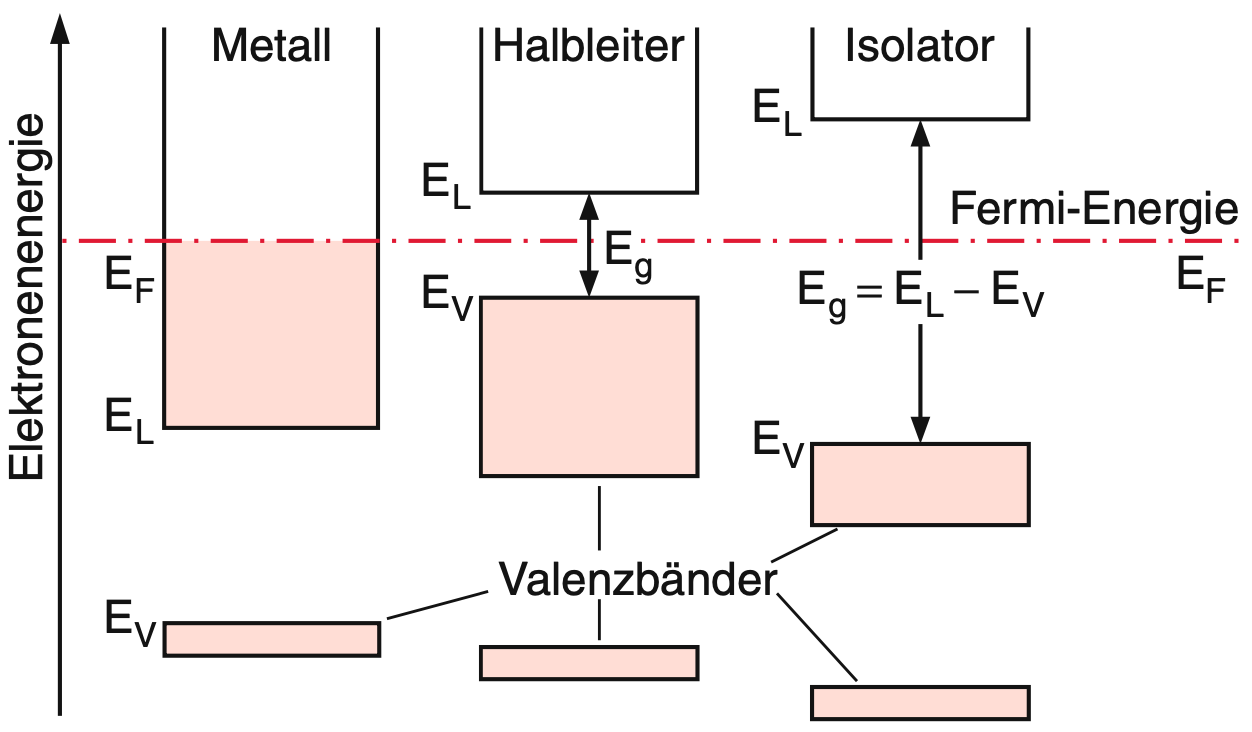
\includegraphics[width=12cm]{fotos/Bandschemata.png}
    \caption{Die Bandschemata von Leitern, Halbleitern und Isolatoren. \cite{demtroeder}}
    \label{fig:Bandschemata}
\end{figure}
Bei Halbleitern ist die elektrische Leitfähigkeit bei tiefen Temperaturen gering. Bei einer Temperatur von $T = \num{0}$ ist das Valenzband voll besetzt und das Leitungsband leer, d.h. sie sind Nichtleiter. Die Bandlücke bei Halbleitern ist geringer als die Bandlücke bei Isolatoren. \cite{demtroeder}
Die Fermi-Energie $E_F$ liegt bei $T = \num{0}$ in der Mitte der verbotenen Zone zwischen Valenz- und Leitungsband. Dort ist die Zustandsdichte $D(E)$ Null (siehe Abb. \ref{fig:Leitfähigkeit})

\begin{figure}
    \centering
    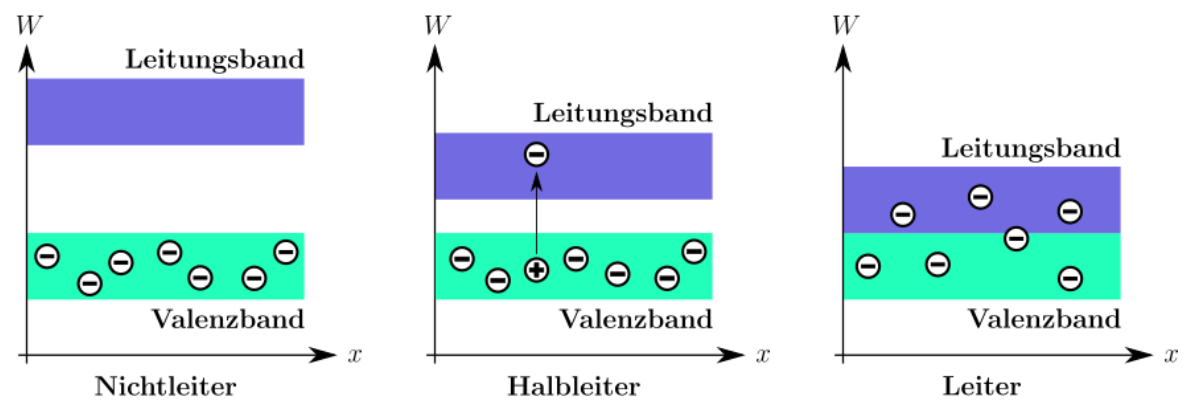
\includegraphics[width=12cm]{fotos/Bandschemata2.png}
    \caption{Noch mal die Bandschemata von Leitern, Halbleitern und Isolatoren. Die Abbildung im Protokoll weglassen. Quelle: Wikipedia}
    \label{fig:Bandschemata2}
\end{figure}

Die Fermi-Verteilung gibt an, welche Energie E ein Fermion bei Temperatur T hat. Bei $T > \num{0}$ reicht die Fermi-Verteilung ins Leitungsband hinein. Die Konzentration der freien Leitungselektronen und damit die elektrische Leitfähigkeit steigen also mit $T$. Schematisch ist das in Abb. \ref{fig:Leitfähigkeit} zu sehen. \cite{demtroeder} %etwas zu sehr wörtlich aus der Quelle abgeschrieben

\begin{figure}
    \centering
    \includegraphics[width=12cm]{fotos/Leitfähigkeit.png}
    \caption{Die von der Temperatur abhängige Fermi-Verteilung und Konzentration der Ladungsträger bei Halbleitern ist zu sehen. \cite{demtroeder}}
    \label{fig:Leitfähigkeit}
\end{figure}

Ein Elektron, das ins Leitungsband gelangt, lässt im Valenzband ein Loch zurück. Die fehlende negative Ladung erscheint als positive Ladung. \cite{demtroeder}

%Konzept der effektiven Masse von freien Ladungsträgern in Festkörpern:
Die effektive Masse von Elektronen im Leitungsband bzw. von Löchern im Valenzband ist gegeben durch
\begin{equation}
    m_\text{eff} = \hbar^2 \cdot \left( \frac{d^2 E}{dk_i \, dk_j} \right)^{-1}.
    \label{eq:m_eff}
\end{equation}
Die effektive Masse hat Tensorcharakter und gibt die inverse Krümmung der Dispersionsrelation $E(k)$ an. \cite{demtroeder}
Die effektive Masse wird eingeführt, um Elektronen wie freie Ladungsträger behandeln zu können. Das heißt der Einfluss des Potentials, das das Elektron im Kristall erfährt, wird berücksichtigt. Unter dem Einfluss einer äußeren Kraft in einem äußeren elektrischen Feld ändert sich zusätzlich zur kinetischen Energie auch die potenzielle Energie des Elektrons. Ein Elektron wird hier als Wellenpaket beschrieben und seine Geschwindigkeit als Gruppengeschwindigkeit dieses Pakets. \cite{demtroeder}

\subsection{Dotierung von Halbleitern}
%Warum ist Dotierung nötig?
Dotierte Halbleiter sind reine Halbleiter, in die ein Fremdatom eingesetzt wird, z.B. indem der Kristall in Dampf der Fremdatome gebracht wird. Die Fremdatome wirken als Störstellen. \cite{demtroeder}
Durch die Dotierung können gezielt Eigenschaften des Halbleiters wie die elektrische Leitfähigkeit geändert werden. (Quelle: Wikipedia)
%noch was?


%Rolle der Donatoren und Akzeptoren, ihre Energieniveaus im Banddiagramm:
Werden fünfwertige (Wertigkeit = Anzahl der Bindungen, die ein Atom eingehen kann) Fremdatome in einen Kristall aus vierwertigen Atomen eingebaut, ist das fünfte Hüllenelektron über viele Gitterplätze delokalisiert und kann als frei angesehen werden. Die Fremdatome werden deshalb als Donatoren bezeichnet. Der dotierte Halbleiter heißt n-Halbleiter. \cite{demtroeder}
\begin{figure}
    \centering
    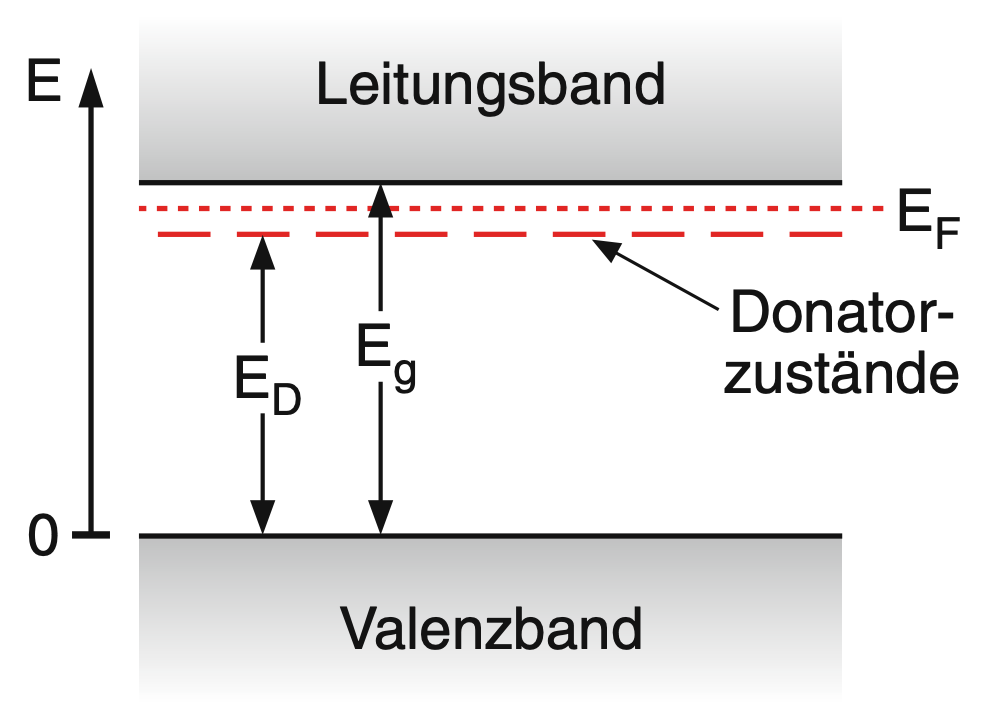
\includegraphics[width=8cm]{fotos/Donator.png}
    \caption{Zu sehen sind die Energieniveaus im Banddiagramm für n-Halbleiter. \cite{demtroeder}}
    \label{fig:donator}
\end{figure}


Werden dreiwertige Fremdatome in einen Kristall aus vierwertigen Atomen eingebaut, bleibt ein freier positiv geladener Platz, in den Elektronen eingefangen werden können. Die Fremdatome werden deshalb Akzeptoren (Elektronenempfänger) genannt. Der dotierte Halbleiter heißt p-Halbleiter. \cite{demtroeder} 
\begin{figure}
    \centering
    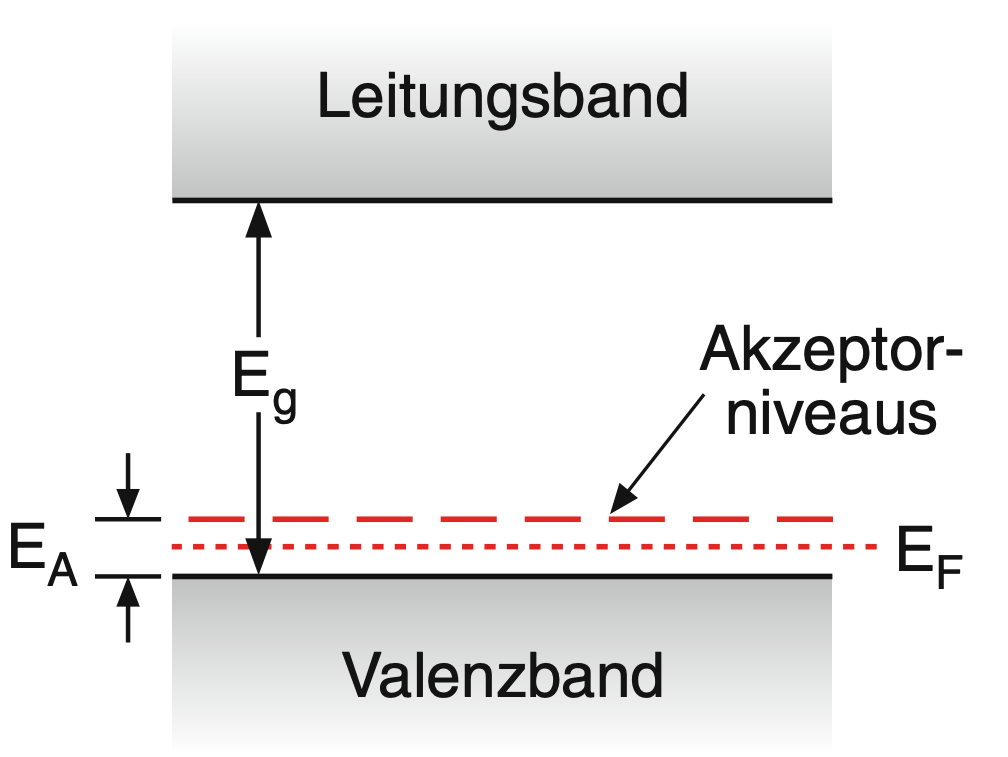
\includegraphics[width=8cm]{fotos/Akzeptor.png}
    \caption{Zu sehen sind die Energieniveaus im Banddiagramm für p-Halbleiter. \cite{demtroeder}}
    \label{fig:akzeptor}
\end{figure}

Bei n-dotierten Halbleitern sinkt die Fermigrenze $E_F$ mit steigender Temperatur $T$, bei p-Halbleitern steigt sie. \cite{demtroeder}

\subsection{Faraday-Effekt}
%Definition des Effekts der Faraday-Rotation
Der Faraday-Effekt beschreibt die Drehung der Polarisationsebene einer linear polarisierten elektromagnetischen Welle in einem Medium, wenn darin ein Magnetfeld parallel zur Ausbreitungsrichtung der Welle herrscht. (Wikipedia)

Die Faraday-Rotation beschreibt die Drehung der Polarisationsebene einer elektromagnetischen Welle in einem Material unter dem Einfluss eines Magnetfeldes, welches parallel zur Ausbreitungsrichtung der Welle ist. (Altprotokoll)

%Phänomenologische Beschreibung


\subsection{Bestimmung der effektiven Masse von Ladungsträgern mithilfe des Faraday-Effekts}
\begin{equation}
    \theta_\text{frei} = \frac{{e_0}^3}{8 \, \pi^2 \, \epsilon_0 \, c^3 \, (m^*)^2} \frac{N \, B}{n} \cdot \lambda^2
    \label{eq:theta}
\end{equation}

%Modell und Ansatz. Wie beeinflusst das Magnetfeld freie Elektronen?
Der Faraday-Effekt/ die Drehung der Polarisationsebene wird durch das Anlegen eines äußeren Magnetfelds erzeugt. Die Elektronen der Materie wechselwirken mit dem Magnetfeld.
Die oben stehende Formel mit m statt $m^*$ gilt für freie Ladungsträger. So gilt sie für Elektronen im Kristall.


\subsection{Detektionstechnik}

\subsection{Alternativer Ansatz zur Detektion}

\subsection{Interferenzfilter und Glan-Thompsen-Prisma}